The ${H_{\infty}}$ control technique is an optimization-based approach composed of two main stages. In the first one, we formulate a minimization norm problem of the closed-loop system between specific signals that we will discuss later on. Then, in the second stage, we solve the optimizazion problem based on the \textit{generalized plant}.
\newline
Our aim is to design a \textit{K} to attenuate the influence of $\omega$ on the signals $z$ in the closed-loop system. In particular, the \textit{generalized plant} has two inputs, $\omega$ and $u$, and two outputs, $z$ and $y$:
\begin{itemize}
	\item \boldmath$\omega$ represents the exogenous input. In our case, it is composed of several signals as the position reference one and the state and measurement noise. As regards the torque disturbances discussed in the frequency domain chapter, we do not consider them because they become significant only when the masses are rotating at steady state. Indeed, in the position control we neglect this behaviour since the masses are stopped after the transient.
	\item \boldmath$u$ is the control input and thanks to it we are able to handle the effect of $\omega$ on $z$.
	\item \boldmath$z$ is the regulated output, which are required to be kept \textit{small}. This signal is so made by the output of the shaping functions, that we will describe later on.
	\item \boldmath$y$ is the measured output and thanks to it the system is able to obtain the information about the effect of $\omega$.
\end{itemize}

\section{1-DOF }
The system is made by four states and two sensors, that are a potentiometer and an encoder. Their noises are respectively indicated as vectors $n_x$ of dimension 4 and $n_y$ of dimension 2. Indeed, $\omega$ will be of dimension 7:

\begin{equation}
	\omega^{T} =
	\begin{bmatrix}
		\theta_{1_{ref}} & n_x & n_y
	\end{bmatrix}
\end{equation}

Considering the state and measurement noises written above, we need to specify their variances. The state ones ($\tilde{Q}$) are obtained through an empirical tuning, while the sensors ones ($\tilde{R}$) are computed with methods discussed in the first chapter of the report. The matrices are so composed:

\begin{equation}
	\tilde{Q}=
	\begin{bmatrix}
		0.3*10^{-4} & 0 & 0 & 0 \\
		0 & 10^{-2} & 0 & 0 \\
		0 & 0 & 10^{-8} & 0 \\
		0 & 0 & 0 & 10^{-4}
	\end{bmatrix}
	\\
	\tilde{R}=
	\begin{bmatrix}
		10^{-6} & 0\\
		0 & 2*10^{-8} & 
	\end{bmatrix}	
\end{equation}

From these matrices, it is possible to notice how we trust more the position state (first and third state) with respect the speed ones. Moreover, we consider more reliable the encoder measurement than the potentiometer one and this is reflected also on $\tilde{Q}$. 
\newline
We are going to build now the \textit{generalized plant} $P(s)$.
\begin{equation}
	P(s)
	=
	\left[
	\begin{array}{c|cc}
		A & B_{\dot{x}\omega} & B \\
		\hline
		C & D_{y\omega} & D	
	\end{array}
	\right]
\label{P(s)}
\end{equation}

where $A$,$B$,$C$ and $D$ are the system matrices, while $B_{\dot{x}\omega}$ and $D_{y\omega}$ are:

\begin{equation}
	B_{\dot{x}\omega}=
	\begin{bmatrix}
		zeros(n_x,1) & \sqrt{\tilde{Q}} & zeros (n_x,n_y)
	\end{bmatrix}
\end{equation}

\begin{equation}
	D_{y\omega}=
	\begin{bmatrix}
		zeros(n_y,1) & zeros (n_y,n_x) & \sqrt{\tilde{R}}
	\end{bmatrix}
\end{equation}

We design now the shaping functions illustrated in \ref{Weighting functions scheme1dof}. For what concerns $W_e$, we prefer to weight more the error at low frequencies to reduce as much as possible its value at steady state. Whereas for $W_u$, we want to limit the bandwidth of the control action, predilecting the low frequencies, not to take the amplifier to its extreme performance. This choice leads us to a less aggressive regulator and so we expect to have some oscillations that the control action is not able to compensate. In order to reduce this behavior, we design an additional shaping function which limits $\theta_{1}$ at high frequencies.

\begin{figure*}[h]
	\centering
	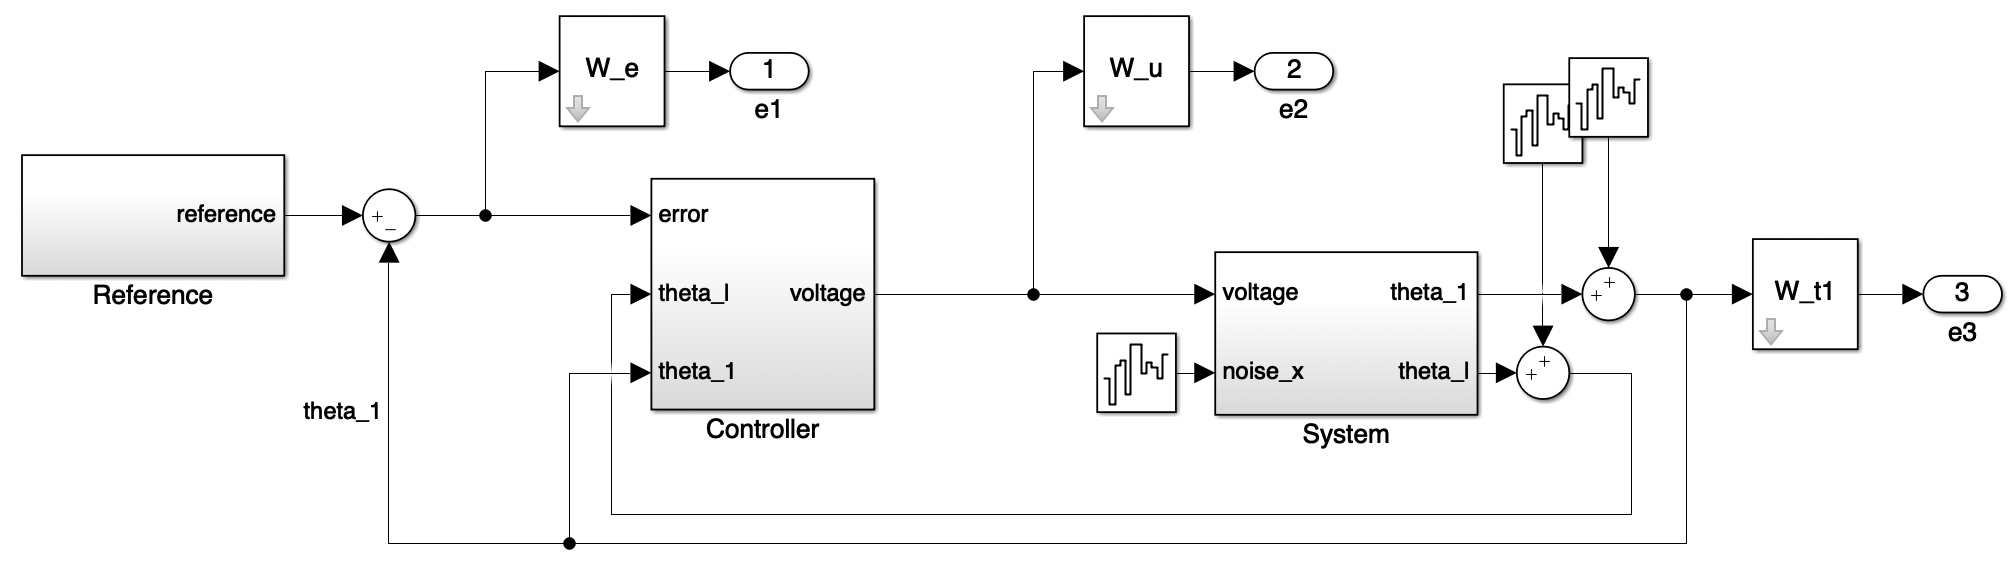
\includegraphics[scale=0.3]{Wfig1dof}
	\caption{Weighting functions scheme}
	\label{Weighting functions scheme1dof}
\end{figure*}
Starting from this reasoning, we tune the weighting function empirically at the laboratory. Below the final choices are shown:

\begin{equation}
	W_e=
	\frac{s+30}{s+0.01}
	\\
	,
	\\
	W_u=
	\frac{s+0.1}{s+150}
	\\
	,
	\\
	W_{\theta_{1}}=
	\frac{s+10}{0.01*s+2}
\end{equation}

\begin{figure*}[h]
	\centering
	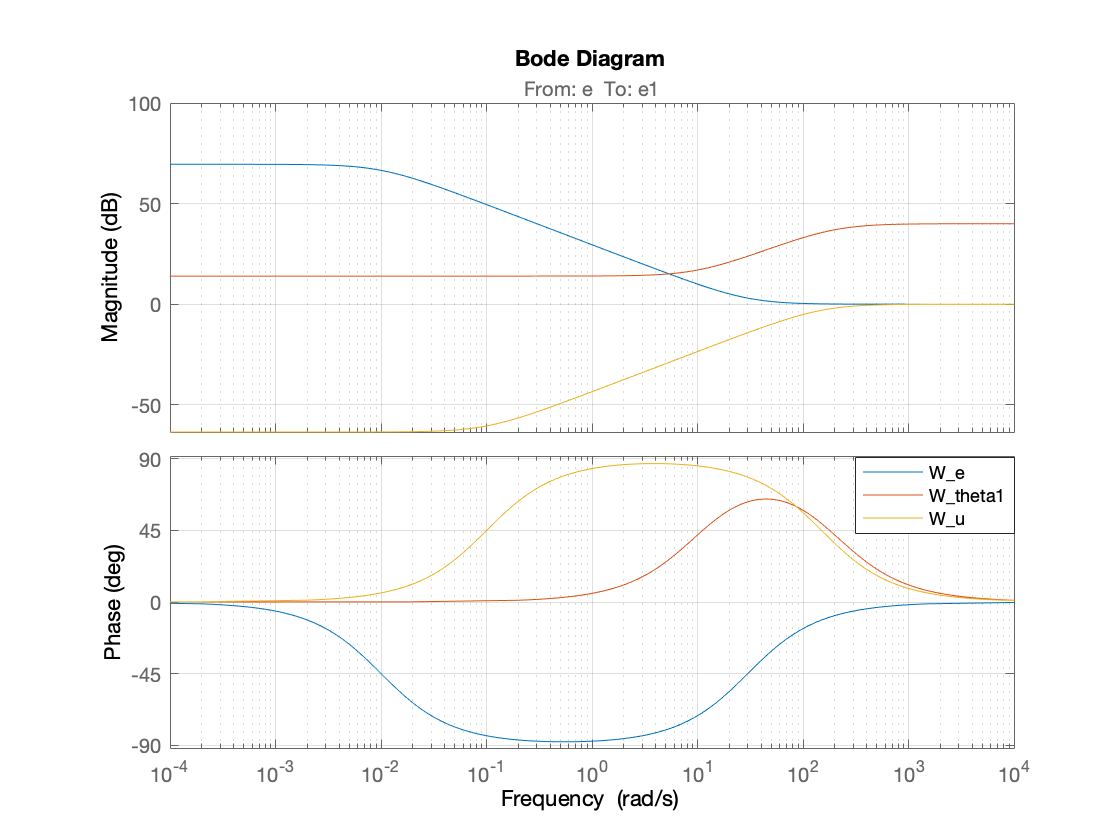
\includegraphics[scale=0.3]{W1dof}
	\caption{Weighting functions}
\end{figure*}

 In figure \ref{fig:posH1dof}, it is observable how the simulation and the laboratory data share the same settling time and this one is the fastest ever obtained throughout the project work. Anyway, the simulation does not model the oscillations arisen in the laboratory and it is for this reason not fully reliable. Furthermore, in both the experiments we are able to reach the reference at steady state.
 
 \begin{figure*}[h]
 	\centering
 	\begin{subfigure}{0.5\columnwidth}
 		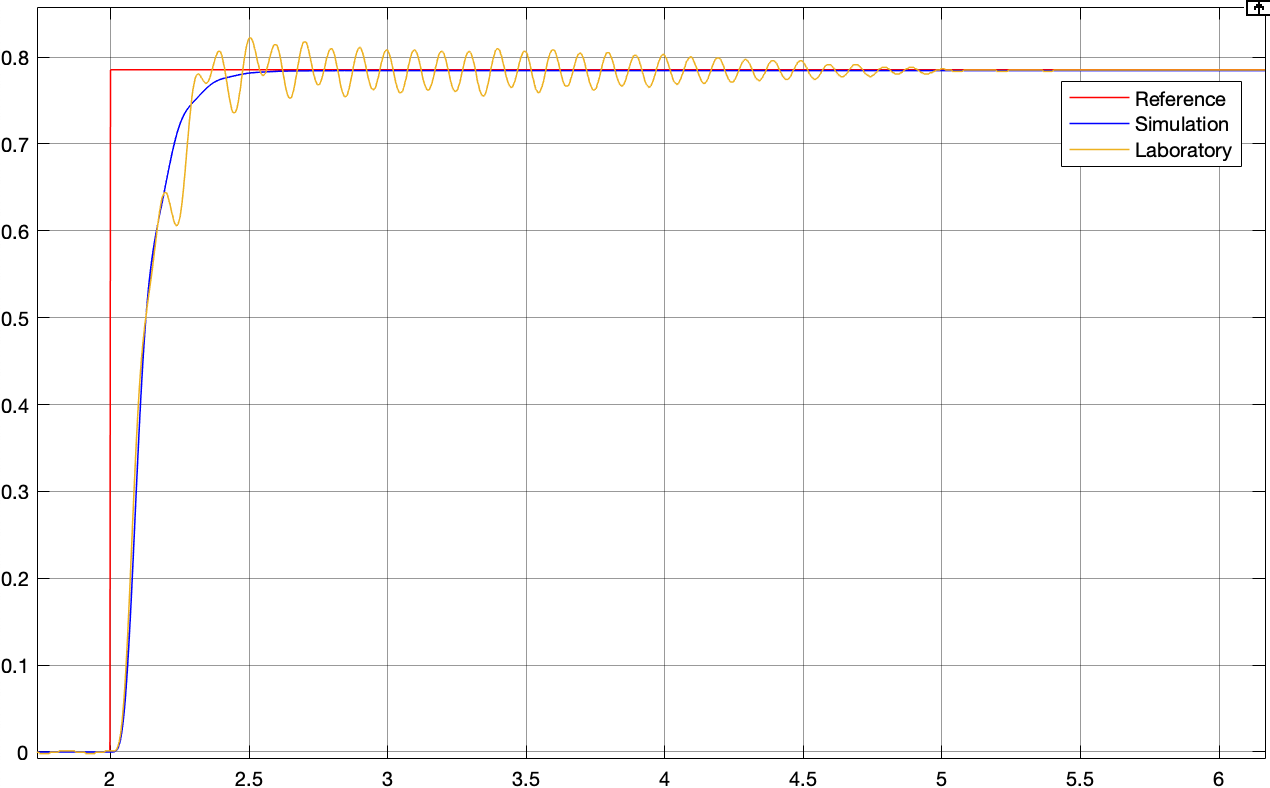
\includegraphics[scale= 0.37]{posH1dof}
 		\caption{Position}
 	\end{subfigure}
 	\begin{subfigure}{0.45\columnwidth}
 		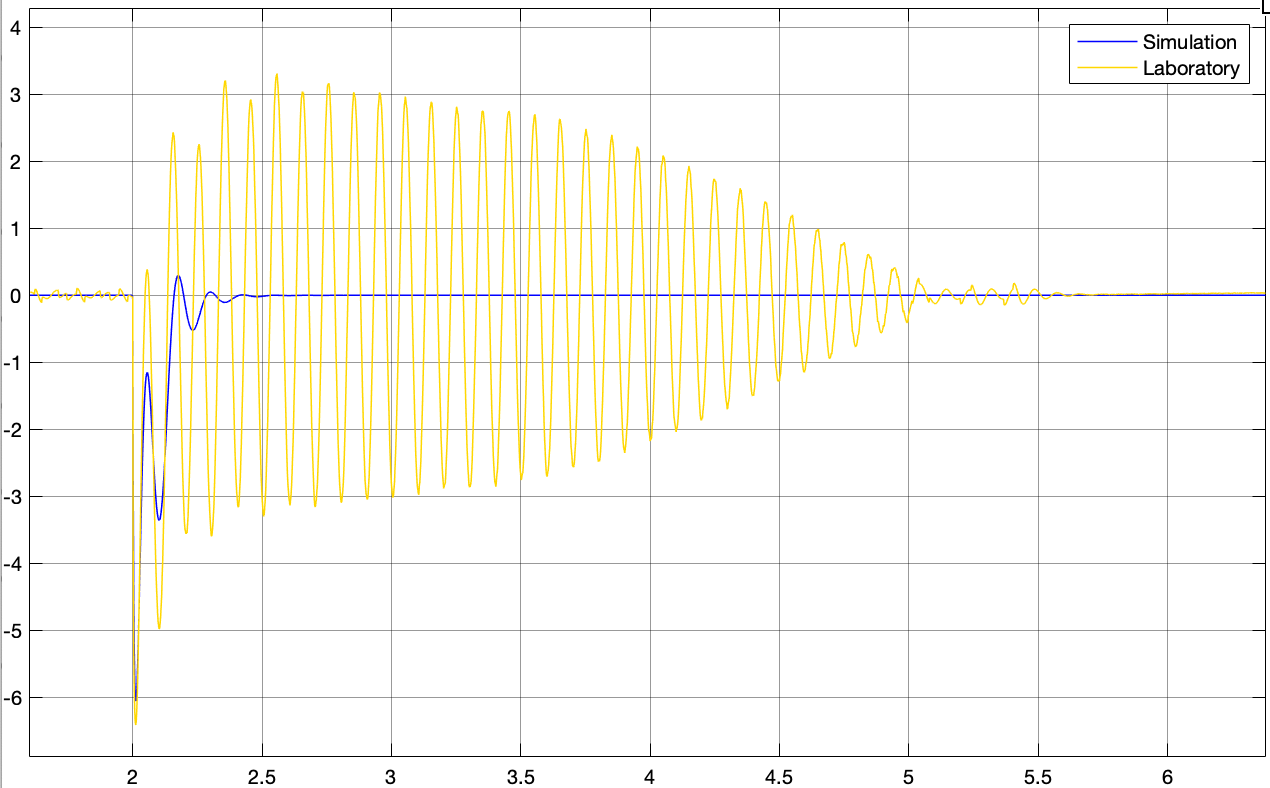
\includegraphics[scale=0.37]{voltH1dof}
 		\caption{Voltage}
 	\end{subfigure}
 	\caption{Position step response}
 	\label{fig:posH1dof}
 \end{figure*}

Due to a lack of time, the final result is not satisfactory, but we suppose that if we could have applied the solution obtained in the 2-DOF case, in which we spent more time, the result would have been acceptable.
\newpage
\section{2-DOF}
In this scenario, the system states are 6 and the sensors are 3, for this reason $\omega$ is composed of 10 signals:

\begin{equation}
	\omega^{T} =
	\begin{bmatrix}
		\theta_{2_{ref}} & n_x & n_y
	\end{bmatrix}
\end{equation}

Coherently with the 1-DOF case, we build the variances matrices keeping the same values:

\begin{equation}
	\tilde{Q}=
	\begin{bmatrix}
		0.3*10^{-4} & 0 & 0 & 0 & 0 & 0\\
		0 & 10^{-2} & 0 & 0 & 0 & 0\\
		0 & 0 & 10^{-8} & 0 & 0 & 0 \\
		0 & 0 & 0 & 10^{-4} & 0 & 0 \\
		0 & 0 & 0 & 0 & 10^{-8} & 0 \\
		0 & 0 & 0 & 0 & 0 & 10^{-4}
	\end{bmatrix}
	\\
	\tilde{R}=
	\begin{bmatrix}
		10^{-6} & 0 & 0\\
		0 & 2*10^{-8} & 0 \\
		0 & 0 & 2*10^{-8} 
	\end{bmatrix}	
\end{equation}

The definition of the \textit{generalized plant} $P(s)$ is the same explained starting from the formula \ref{P(s)}. Then, we go on implementing the following weighting functions:

\begin{figure*}[h]
	\centering
	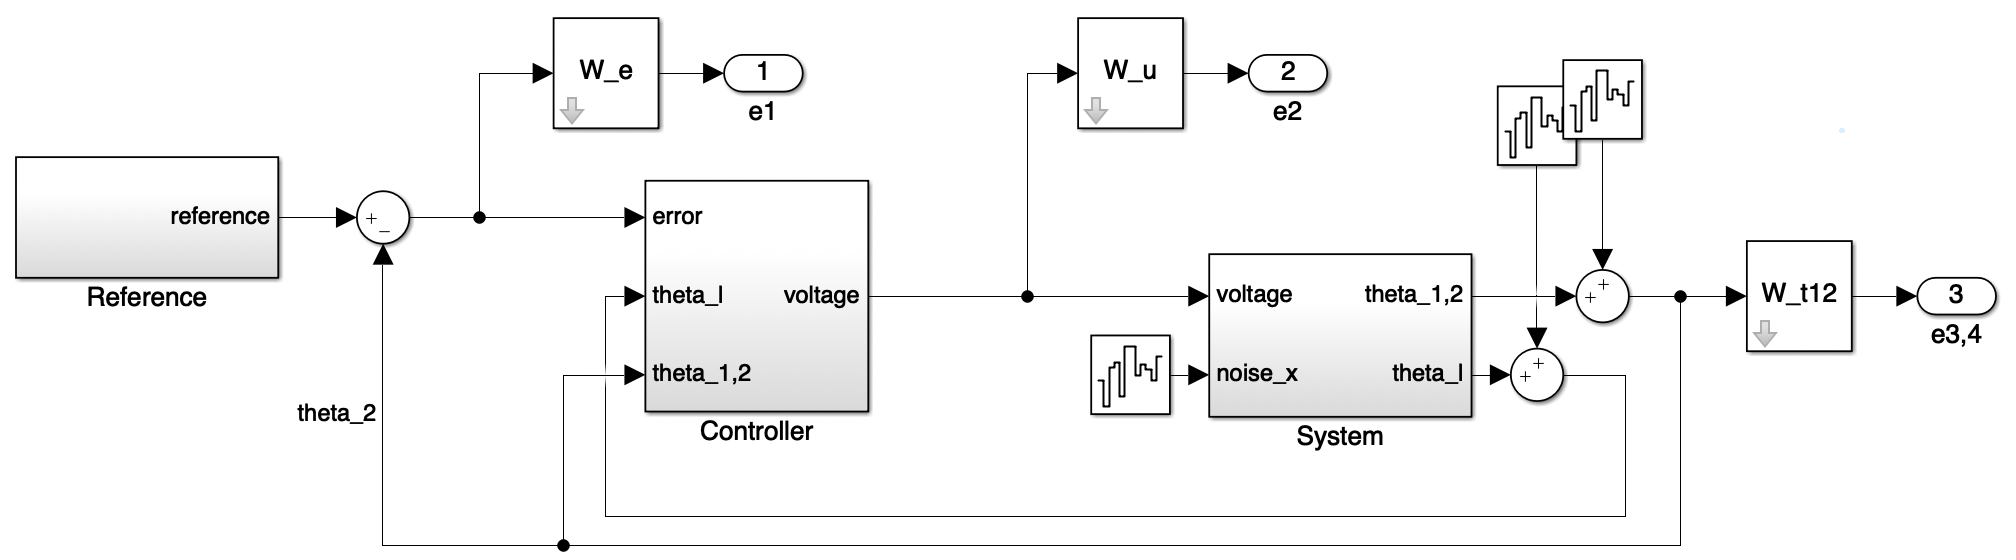
\includegraphics[scale=0.3]{Wfig2dof}
	\caption{Weighting functions scheme}
	\label{Weighting functions scheme2dof}
\end{figure*}

The reasoning followed to design these functions is the same written above and the differences between them are due to a different tuning made at the laboratory. To overcome as possible the oscillation issue, we penalize homogeneously the whole control frequency range. In a first moment we tried to apply just one weighting function $W_{\theta_{2}}$ on the second mass, but then we realized how the first mass was oscillating exceedingly. We choose so to shape another function to penalize the high frequencies of the first mass postion.

\begin{equation}
	W_e=
	\frac{s+30}{2*s+0.02}
	\\
	,
	\\
	W_u=0.9
	\\
	,
	\\
	W_{\theta_{1}}=
	\frac{s+10}{0.01*s+2}
	\\
	W_{\theta_{2}}=
	\frac{s+10}{0.01*s+2}
\end{equation}

\begin{figure*}[h]
	\centering
	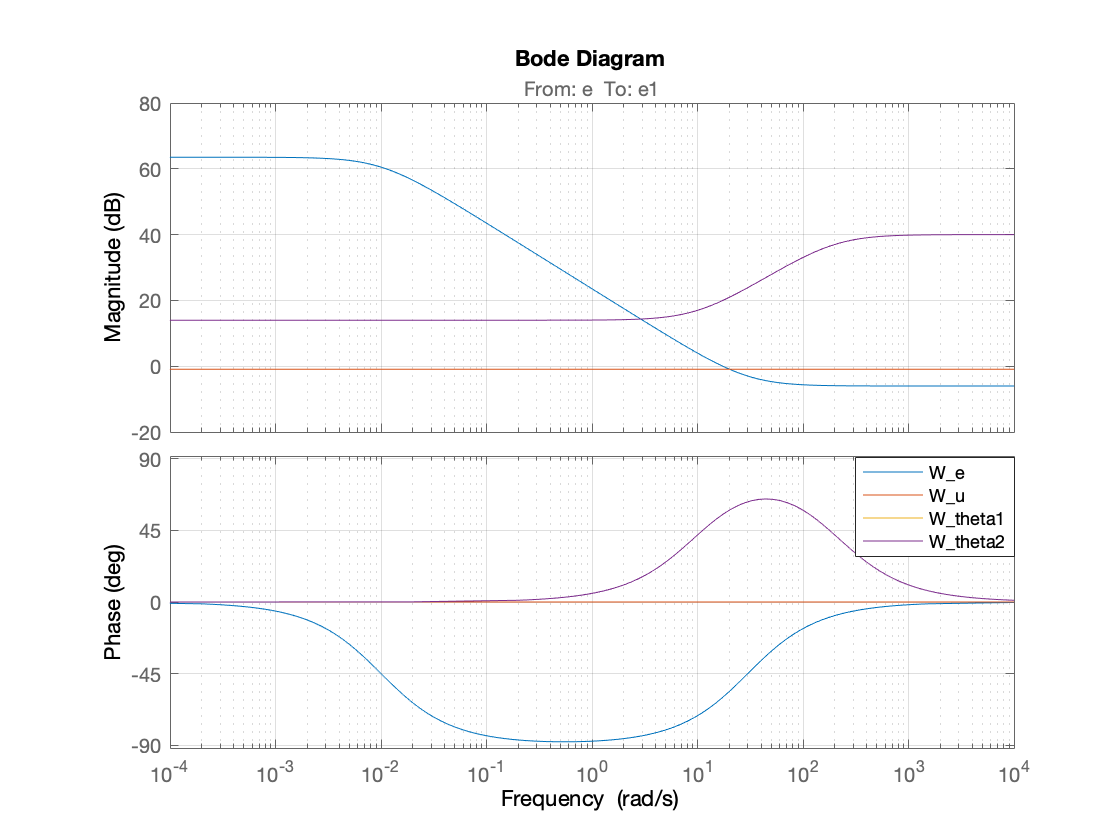
\includegraphics[scale=0.3]{W2dof}
	\caption{Weighting functions}
\end{figure*}

From the plots in figure \ref{fig:posH2dof}, we can notice a significant improvement with respect to the solution of the 1-DOF scenario. Although there are a few oscillations, we can consider this result acceptable. Most likely there exist better solutions, but due to lack of time we did not manage to explore them.

 \begin{figure*}[h]
	\centering
	\begin{subfigure}{0.5\columnwidth}
		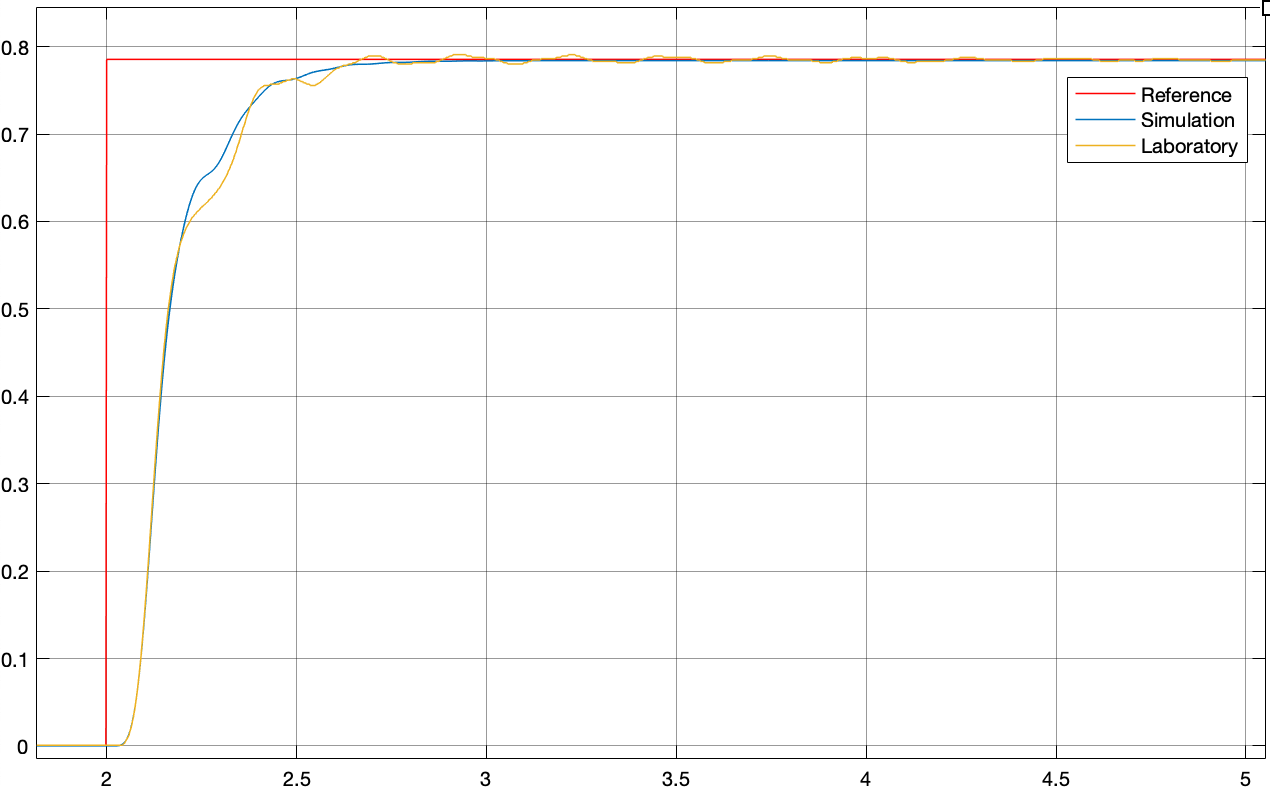
\includegraphics[scale= 0.37]{pi_4H}
		\caption{Position step of $\frac{\pi}{4}$}
	\end{subfigure}
	\begin{subfigure}{0.45\columnwidth}
		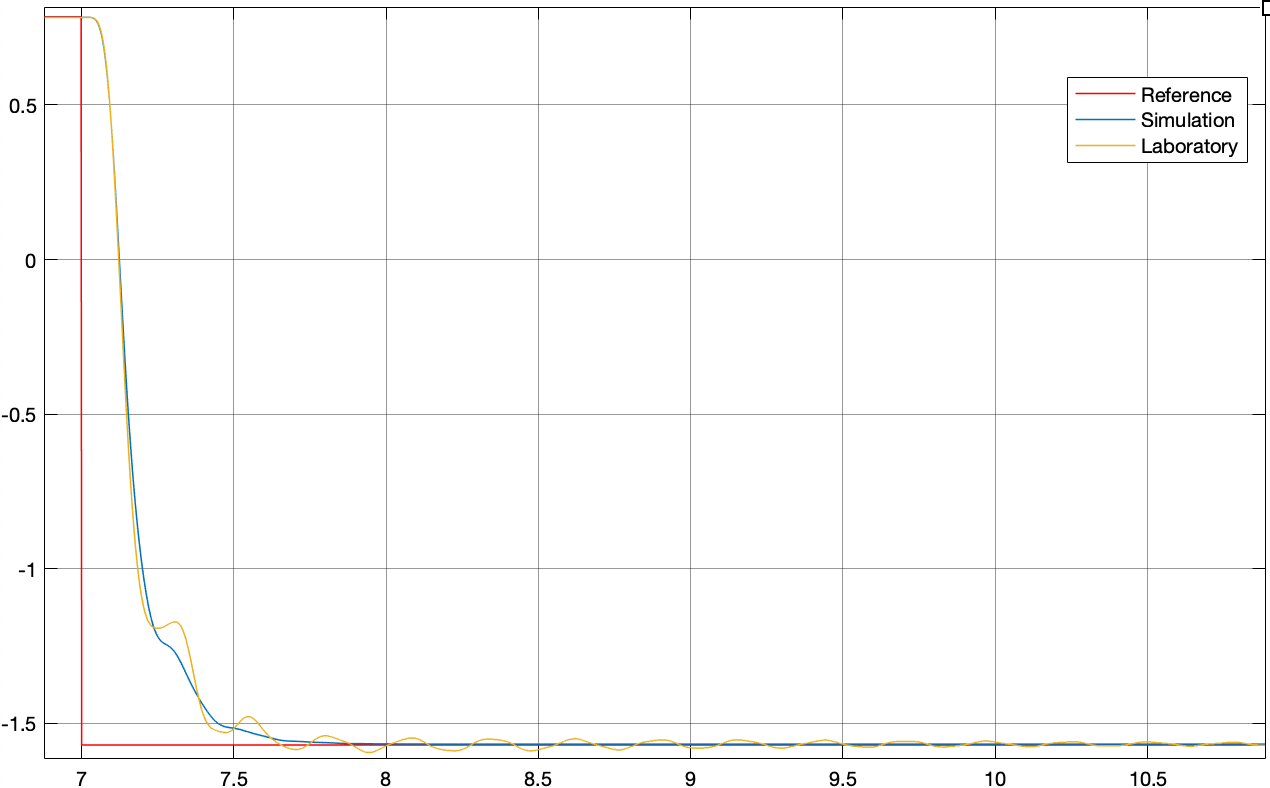
\includegraphics[scale=0.37]{pi_2H}
		\caption{Position step from $\frac{\pi}{4}$ to $-\frac{\pi}{2}$}
	\end{subfigure}
	\\
	\begin{subfigure}{0.5\columnwidth}
		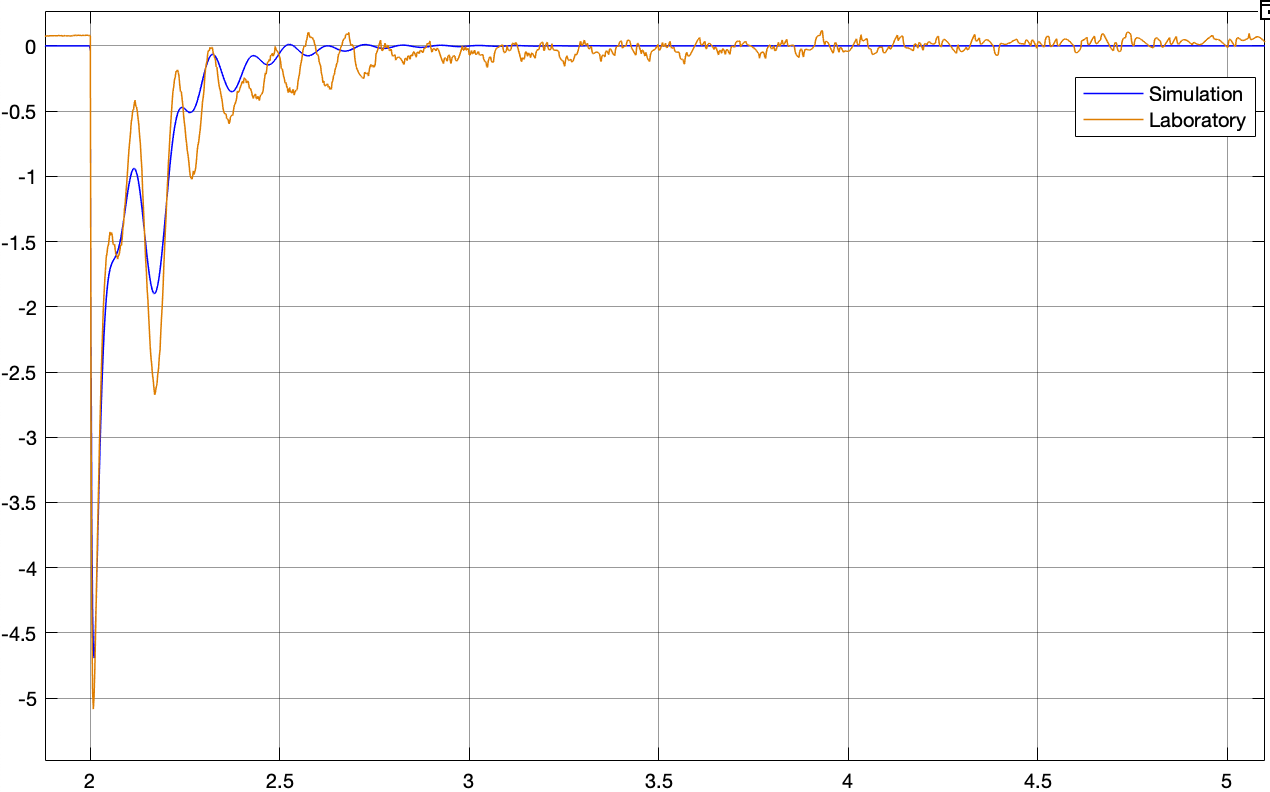
\includegraphics[scale= 0.37]{pi_4Hvolt}
		\caption{Voltage for a step of $\frac{\pi}{4}$}
	\end{subfigure}
	\begin{subfigure}{0.45\columnwidth}
		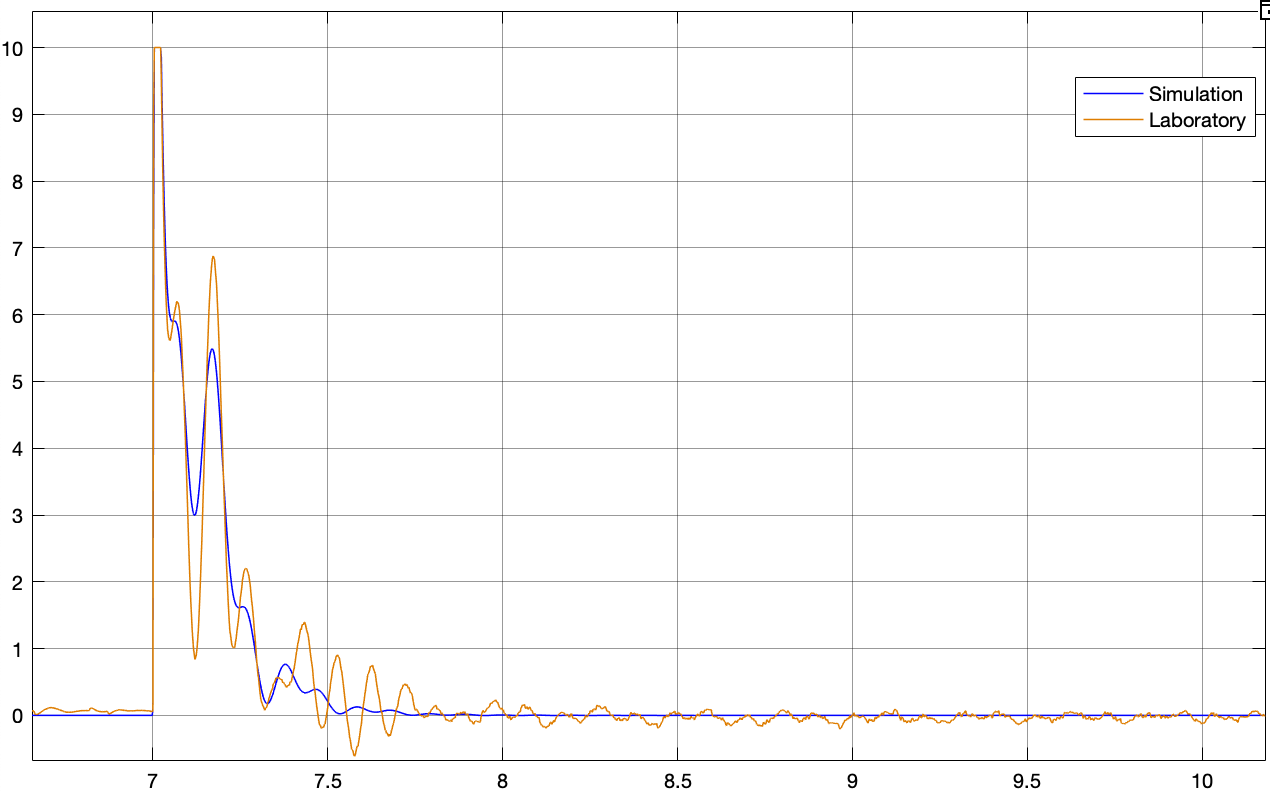
\includegraphics[scale=0.37]{pi_2Hvolt}
		\caption{Voltage for a step from $\frac{\pi}{4}$ to $-\frac{\pi}{2}$}
	\end{subfigure}
	\caption{Position steps response}
	\label{fig:posH2dof}
\end{figure*}




 


